\chapter{Numerical Method}
\label{chapter2}

%--------------------------------------
\section{Mathematical Models and Numerical Method}
\label{sec:equations}

\subsection{Linear Elastic Equation and Weak Galerkin Method}
Consider an elastic body subject to an exterior force $ \mathbf{f} $, we denote the computational domain as $ \Omega $ and its continuous boundary as $ \Gamma = \partial \Omega $. The governing equation for linear elasticity can be written as

\begin{equation}
\nabla \cdot \sigma(\mathbf{u}) = \mathbf{f}, \qquad in \quad \Omega 
\end{equation}
\begin{equation}
\mathbf{u} = \hat{\mathbf{u}}, \qquad on \quad \Gamma
\end{equation}
where $ \sigma(\mathbf{u}) $ is the symmetric Cauchy stress tensor. For linear, isotropic and homogeneous materials, the stress-strain relation is
\begin{equation}
\sigma(\mathbf{u}) = 2 \mu \varepsilon(\mathbf{u}) + \lambda (\nabla \cdot \mathbf{u}) \mathbf{I}
\end{equation}
where $ \varepsilon(\mathbf{u}) = \frac{1}{2} (\nabla \mathbf{u} + \nabla \mathbf{u}^{T}) $, $ \mu $ and $ \lambda  $ are Lame indices which can be written as 
\begin{equation}
\lambda = \frac{E\mu }{(1 + \mu) (1 - 2\mu)}
\end{equation}
\begin{equation}
\mu = \frac{E}{2(1+\mu)}
\end{equation}
where $ E $ is the elasticity modulus and $ \mu $ is the Poisson's ratio.



The weak function on the domain is $ \mathbf{u} = \{\mathbf{u}_0, \mathbf{u}_b \}, \quad \mathbf{u}_0 \in L^{2} (T) $. The first function $ \mathbf{u}_0 $  represents the interior domain of the function $ \mathbf{u} $ . The second function $ \mathbf{u}_b $ represents the value of function $ \mathbf{u} $ on the boundary of domain $ T $ . The key notion is that for two function $ \mathbf{u}_0 $  and $ \mathbf{u}_b $  are independent with each other along . The weak function is defined as
\begin{equation}
V_{h} = \{ \mathbf{v} = \{ \mathbf{v}_0, \mathbf{v}_b \} : \mathbf{v}_0 \in P_{j} (T^0), \mathbf{v}_b \in P_{l}(e), e \subset \partial T\}
\end{equation}

The key of the weak Galerkin method is to approximate the solution in the weak discrete space $ S(T) $. The discrete weak gradient $ \nabla_{w} \mathbf{u} \in [P_{r} (T)]^{d} $ for $ \mathbf{u} \in V_{h} $ on each element $ T $:
\begin{equation}
(\nabla_w \mathbf{u}, \mathbf{q})_{T} = - (\mathbf{u}_0, \nabla \cdot \mathbf{q})_{T} + \langle \mathbf{u}_b, q \cdot \mathbf{n} \rangle_{\partial T}
\end{equation}

For the discrete weak divergence, $ \nabla_{w} \cdot \mathbf{u} \in [P_{r} (T)]^{d} $ is defined
\begin{equation}
(\nabla_w \cdot \mathbf{u}, \mathbf{q})_{T} = - (\mathbf{u}_0, \nabla  \mathbf{q})_{T} + \langle \mathbf{u}_b \cdot \mathbf{n}, q  \rangle_{\partial T}
\end{equation}

Then we can define the weak strain tensor by using the weak gradient
\begin{equation}
\varepsilon_{w} (\mathbf{u})  = \frac{1}{2} (\nabla_w  \mathbf{u} + \nabla_w  \mathbf{u}^T)
\end{equation}

Analogously, we can define the weak stress tensor as
\begin{equation}
\sigma_{w} ( \mathbf{u}) = 2 \mu \varepsilon_{w} ( \mathbf{u}) + \lambda (\nabla_w \cdot  \mathbf{u}) \mathbf{I}
\end{equation}

The bilinear form of governing equation of continuous Galerkin method is following
\begin{equation}
a( \mathbf{u},  \mathbf{v}) = ( \mathbf{f},  \mathbf{v})
\end{equation}

The above approximation function $  \mathbf{u} $ and gradient $ \nabla \mathbf{u} $ is not well defined for the discontinuous feature of weak Galerkin method, the new form is 
\begin{equation}
a( \mathbf{u}_w,  \mathbf{v}_w) + s( \mathbf{u},  \mathbf{v}) = ( \mathbf{f},  \mathbf{u})
\end{equation}
the term $ s( \mathbf{u},  \mathbf{v}) $ is a stabilizer enforcing a weak continuity which measures the discontinuity of the finite element solution. The governing equation in weak form can be introduced by two bilinear equations
\begin{equation}
s( \mathbf{u},  \mathbf{u}) = \sum_{T\in \Omega}^{N} h_{T}^{-1} \langle Q_{b}  \mathbf{u}_0 -  \mathbf{u}_b, Q_b  \mathbf{v}_0 -  \mathbf{v}_b \rangle_{\partial T}
\end{equation}
where $ Q_b $ is the projection from the interior unknown variables to boundary unknown variables. Commonly it is taken as $ 1 $. The discrete bilinear equation has the assemblage form
\begin{equation}
a( \mathbf{u}_w,  \mathbf{u}_w) = \sum_{T \in \Omega}^{N} 2(\mu \varepsilon_w ( \mathbf{u}), \varepsilon_w ( \mathbf{v}))_T + \sum_{T \in \Omega}^{N}(\lambda \nabla \cdot \mathbf{u}, \nabla_w \cdot \mathbf{v})_T
\end{equation}


%--------------------------------------
\section{Existing Numerical Methods Review}
In this section, we present and analyze several most widely used numerical method to solve finite element problems. The details of each method are presented in the following subsections. 
\subsection{Classic Continuous Galerkin Finite Element Method}
Back to 1950s and 1960s, finite element method is arised to solve complex elasticity and structural analysis engineering problems in mechanical and aeronautical field. A. Hrennikoff\cite{hrennikoff1941solution}, R. Courant\cite{courant1994variational} and K.Feng are the earliest pioneers who established this subject. FEM is then proposed as a systematic numerical method to solve variety of partial differential equations. The core characteristic of FEM is that it employs mesh discretization to divide a continuous computational domain so that a big problem is then converted to a set of discrete small problems. That is the source of finite element. Each element represents a small piece of computational sub-domain.

Finite element method is an efficient solution to solve partial differential equations. The core idea is to convert the original partial differential equation to a equivalent bilinear form weak function. Then we partition the computational domain into polygon meshes. In each mesh element, we construct the finite element space. Then the bilinear form is discretized into a summation of finite elemental spaces. The solution is approximated based on the calculation of assembled matrix. More details can be found in \cite{zienkiewicz1977finite, ciarlet2002finite, hughes2012finite, reddy1993introduction}

The variational formulation which generated by the governing equation determines the characteristic of the finite element method. To obtain the variational form, many mathematicians derived several different paths such as Galerkin method, the discontinuous Galerkin method, mixed method, etc. In this chapter, we introduce two most popular method, DG and MFEM. The WG method is inspired from these two method and shares many similarities with them. 

\subsection{Discontinuous Galerkin Finite Element Method}


\subsection{Mixed Finite Element Method}



%---------------------------
\section{Weak Galerkin Finite Element Methods}
\subsection{Weak Galerkin triangular meshes}

Consider triangular element linear type basis function for both interior and boundary subspaces $ P_{1}(T) / P_{1} (\partial T) $
\begin{equation}
\phi_{k} = \{ \lambda_{k}, 0 \}, \qquad k = 1,2, 3
\end{equation}
\begin{equation}
\phi_{3 + l} = \{ 0, \mu_{l} \}, \qquad l = 1, 2, \cdots , 2N
\end{equation}
where N is the number of element boundaries.

\begin{figure}[h]
	\centering
	\begin{tabular}{c}
		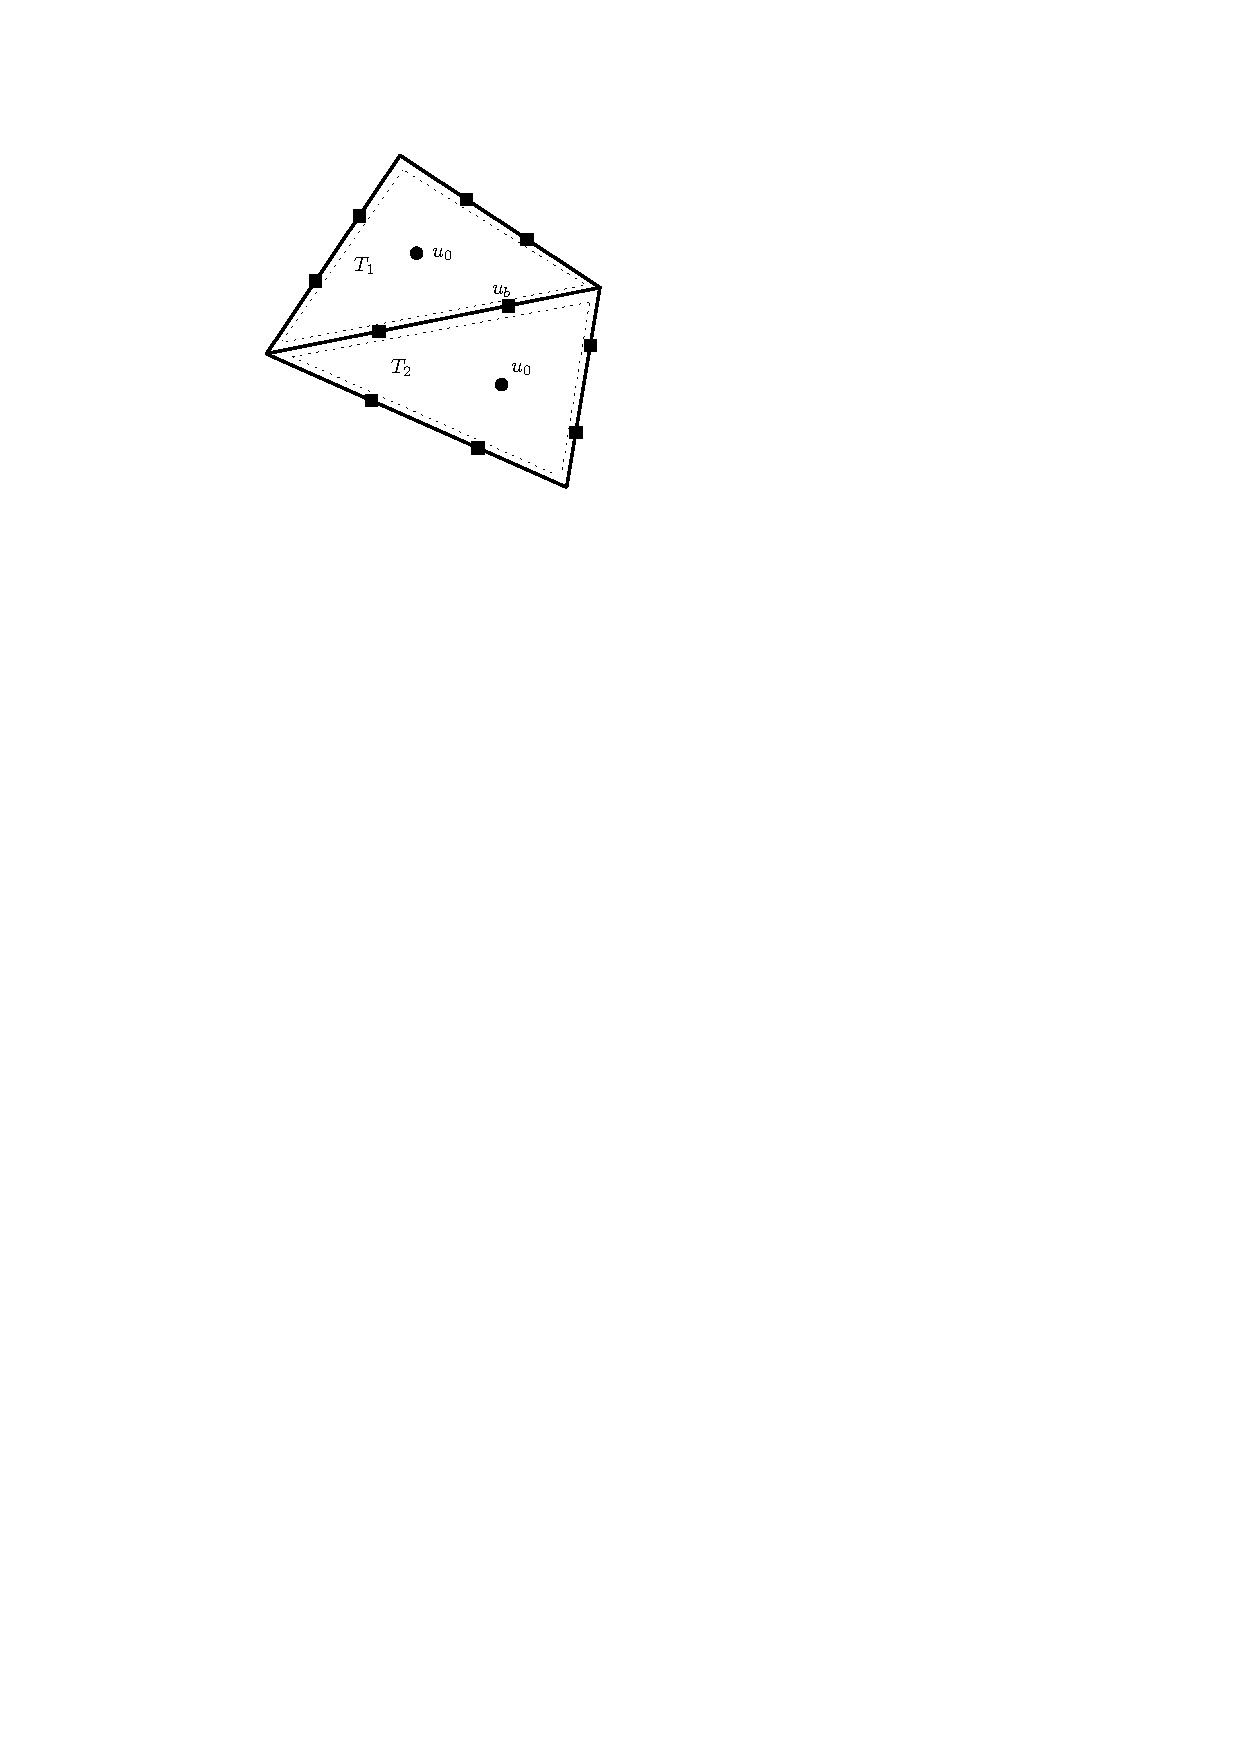
\includegraphics[width=0.5\textwidth]{./pics/triangle.pdf}
	\end{tabular}
	\caption{\footnotesize Weak Galerkin triangular elements and solution points.}\label{fig1: triangle}
\end{figure}

\subsection{Weak Galerkin quadrilateral meshes}

Consider triangular element linear type basis function for both interior and boundary subspaces $ Q_{1}(T) / Q_{1} (\partial T) $
\begin{equation}
\phi_{k} = \{ \lambda_{k}, 0 \}, \qquad k = 1,2, 3
\end{equation}
\begin{equation}
\phi_{3 + l} = \{ 0, \mu_{l} \}, \qquad l = 1, 2, \cdots , 2N
\end{equation}
where N is the number of element boundaries.
\begin{figure}[h]
	\centering
	\begin{tabular}{c}
		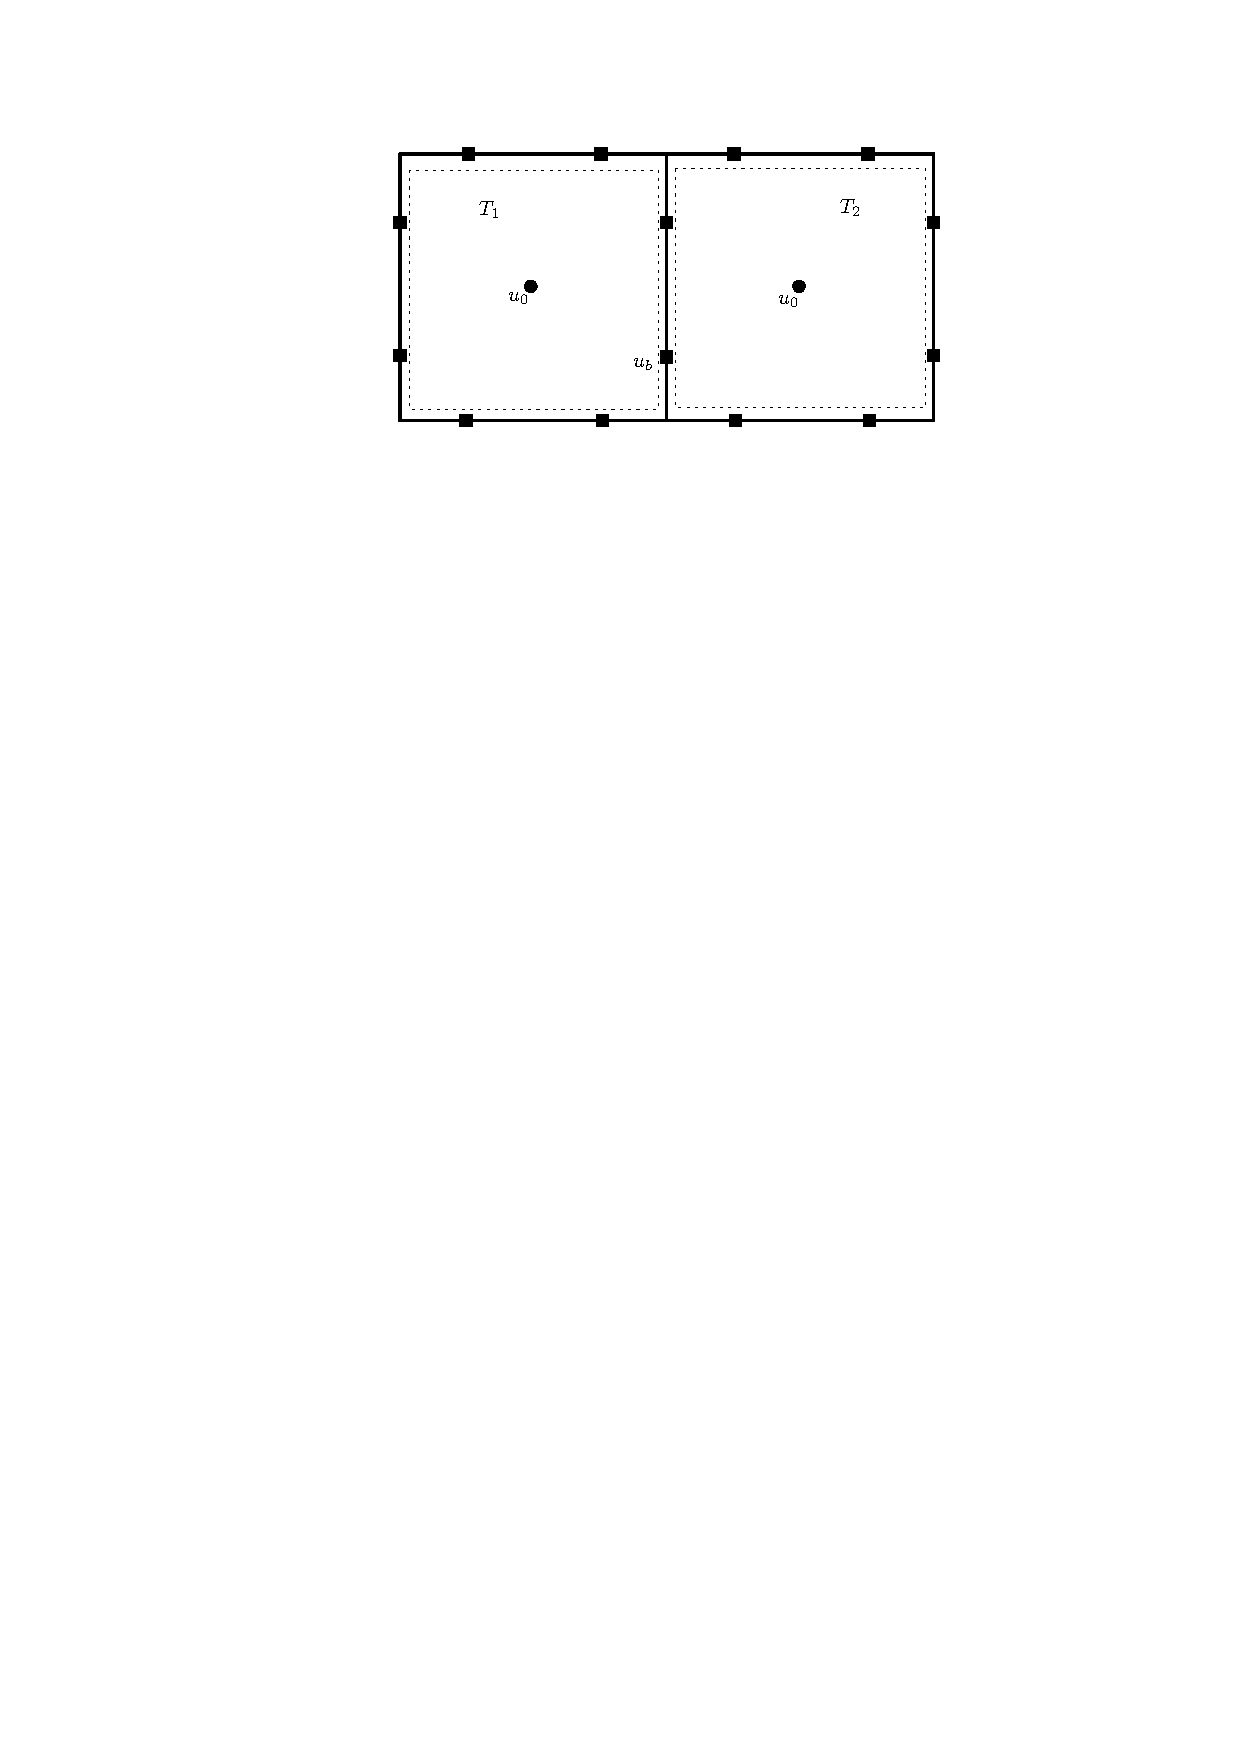
\includegraphics[width=0.8\textwidth]{./pics/quad.pdf}
	\end{tabular}
	\caption{\footnotesize Weak Galerkin quadrilateral elements and solution points.}\label{fig2: quad}
\end{figure}

%--------------------------
